\documentclass{beamer}
\usetheme{Singapore}
\hypersetup{pdfpagemode=FullScreen}

\title{The Examined Life}







\subject{Why Philosophy?}



\AtBeginSection{\frame{\sectionpage}}
\AtBeginSubsection{\frame{\subsectionpage}}
\AtBeginSubsubsection{\frame{\subsubsectionpage}}


\begin{document}


\begin{frame}
\titlepage
\end{frame}

\section{Why Philosophy?}
\frame{
\begin{block}{Red Pill or Blue Pill?}
\url{https://www.youtube.com/watch?v=zE7PKRjrid4}
\end{block}
\begin{block}{Discuss}
\begin{itemize}
\item Could you live an authentic life in the Matrix? Give reasons
for your answer.
\item  Which pill would you take? Why?
\end{itemize}
\end{block}
}

 
 \section{Philosophy Pays}
 
   \frame{\frametitle{George Soros}
\begin{center}
       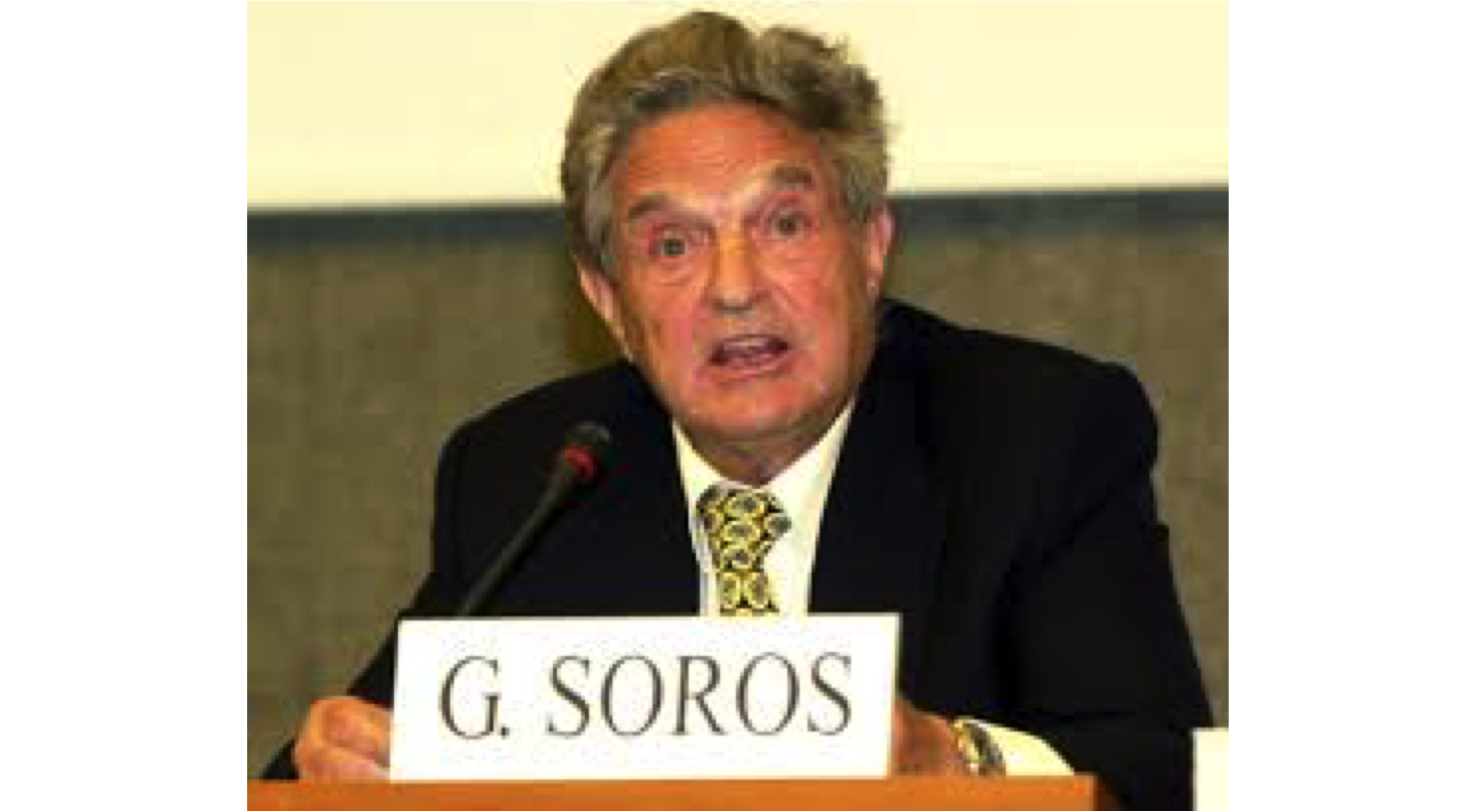
\includegraphics[width=\textwidth, height=6cm]{soros.png}
      \end{center}
}
 
 
%   \frame{\frametitle{Carl Icahn}
%\begin{center}
 %      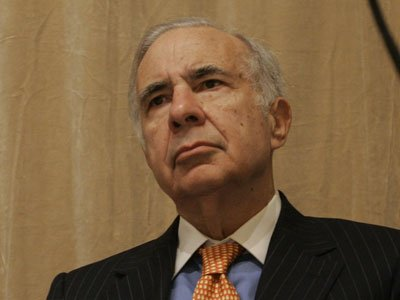
\includegraphics[width=\textwidth, height=7cm]{icahn.jpg}
  %    \end{center}
%}
 
   \frame{\frametitle{Carly Fiorina: HP CEO} 
\begin{center}
       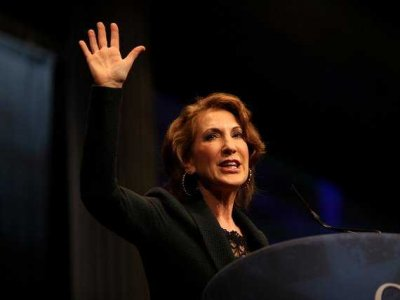
\includegraphics[width=\textwidth, height=7cm]{fiorina.jpg}
      \end{center}
}
 
  \frame{
\begin{center}
       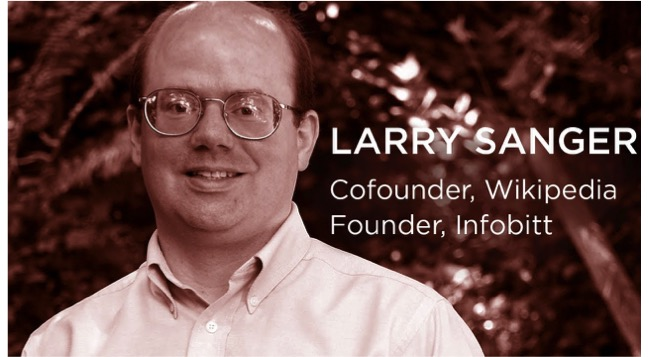
\includegraphics[width=\textwidth, height=7cm]{wikipedia.jpg}
      \end{center}
}
 
  \frame{\frametitle{Peter Thiel: Founder of PayPal}
\begin{center}
       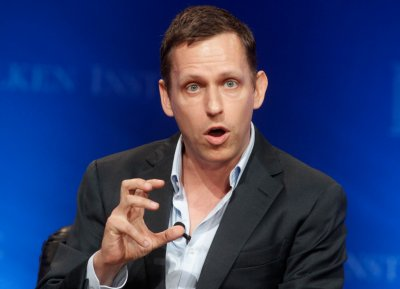
\includegraphics[width=\textwidth, height=7cm]{thiel.jpg}
      \end{center}
}

\frame{\frametitle{Salaries}
\url{http://online.wsj.com/public/resources/documents/info-Degrees_that_Pay_you_Back-sort.html}
}

\section{Philosophy Makes You Smart}

\frame{\frametitle{GMAT}
\url{http://www.nmu.edu/sites/DrupalPhilosophy/files/UserFiles/Files/Pre-Drupal/SiteSections/Resources/GMAT_by_Intended_Major.pdf}
}

    \frame{\frametitle{GRE}
\begin{center}
       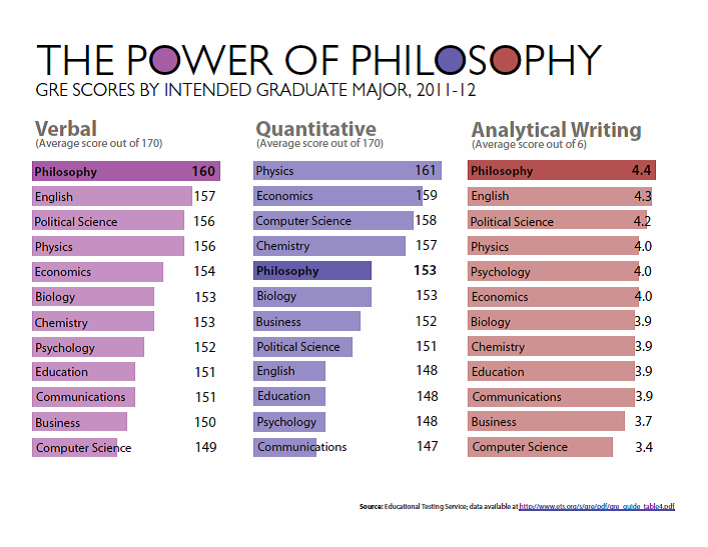
\includegraphics[width=\textwidth, height=7.5cm]{philosophyGRE.png}
      \end{center}
}


\frame{\frametitle{LSAT}
\url{http://www.potsdam.edu/academics/AAS/Phil/upload/LSAT-Scores-of-Majors.pdf}
}

\section{How Philosophy Helps}

\frame{
\begin{block}{3 Important Skills}
\begin{enumerate}
\item The ability to think logically, critically, and independently.
\item The ability to communicate clearly and effectively.
\item The ability to reason with abstract concepts and apply abstract concepts to particular cases. 
\end{enumerate}
\end{block}
}

\frame{\frametitle{Logic: The Math of Critical Thinking}
\begin{block}{}

\begin{itemize}
\item $\exists x(Fx \wedge \forall y(Fy\implies x=y)$
\item $\exists x \exists y((Fx \wedge Gy) \wedge \neg(x=y)) \wedge \forall z(Fz\implies( (z=x \lor z=y))$
\end{itemize}
\end{block}
}

%\frame{\frametitle{Applied to Abstract Material}
%\begin{enumerate}
%\item God is the greatest possible being that can be imagined.
%\item God exists as an idea in the mind.
%\item A being that exists as an idea in the mind and in reality is greater than a being that exists only as an idea in the mind.
%\item Thus, if God exists only as an idea in the mind, then we can imagine something that is greater than God.
%\item But we cannot imagine something that is greater than God (for it is a contradiction to suppose that we can imagine a being greater than the greatest possible being that can be imagined.)
%\item Therefore, God exists.
%\end{enumerate}
%}



\section{The Intrinsic Value of Philosophy: Liberation}

\frame{

\url{https://www.youtube.com/watch?v=69F7GhASOdM}

}

\frame{
\begin{center}
     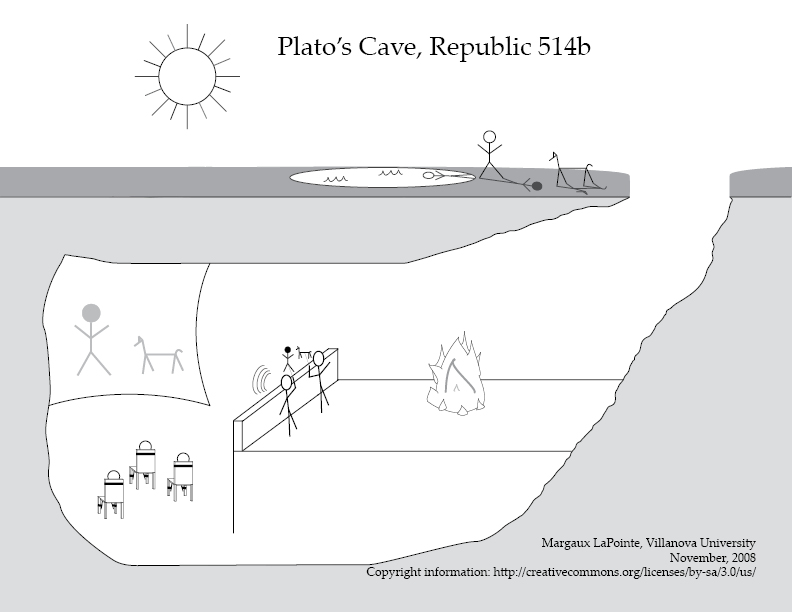
\includegraphics[width=\textwidth, height=7cm]{Cave.jpg}
    \end{center}
}

\frame{
\begin{enumerate}
\item My life has meaning only if God exists. 
\item Suicide is never the best choice. 
\item Knowing that I would live just one more day would not undermine my ability to enjoy that day.
\item God exists and watches over me.
\item There is a heaven.
\item It is wrong to criticize other cultures. 
\item It is wrong to judge other people's actions. 
\item The moral principles that I was raised to believe are the right ones. 
\item I make free choices; all my choices are up to me. 
\item My future is completely determined by my past. 
\end{enumerate}
}

\frame{
\begin{block}{Fundamental vs. Non-Fundamental Beliefs}
\begin{itemize}
\item Your fundamental beliefs are the ones that you use to support other non-fundamental beliefs. 
\item Let us consider two examples, one about health, the other about relationships.
\end{itemize}
\end{block}
}


 
 \frame{ 
\begin{block}{Reflection Time}
\begin{itemize} 
\item List down some of your fundamental beliefs and how they support some of your non-fundamental beliefs.
\end{itemize}
\end{block}
\begin{block}{Where did these beliefs come from?}
\begin{itemize}
\item Can you recall acquiring these beliefs from serious reflection? 
\item Are these beliefs really your own? 
\item Would you have chosen these beliefs if you had been given a choice before they were imposed upon you?  
\item Why do you want to hold on to them?
\end{itemize}
\end{block}
}

   \frame{
   \begin{block}{Liberation}
      \begin{itemize}
      \item Philosophy teaches us 1) how to investigate the compatibility between our non-fundamental and fundamental beliefs, that is, it teaches us how to identify what our fundamental beliefs require of us. 2) It teaches us how to investigate our fundamental beliefs.  
   \item As such, philosophy frees us from a sort of dogmatism that would otherwise overtake our minds by passively holding beliefs that we have never examined.
   \item As a result, we become freed from the beliefs that have been forced upon us and come to possess beliefs that we can truly call our own. 
  
   \end{itemize}
\end{block}
}

%\section{First Few Topics}

%\frame{Critical Thinking
%\begin{center}
 % \includegraphics[width=\textwidth, height=7cm]{}
  %  \end{center}
%}

%\frame{
%\begin{center}
   %  
\includegraphics[width=\textwidth, height=7cm]{purpose.jpg}
    %\end{center}
%}

%\frame{
%\begin{center}
   %  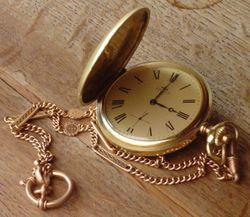
\includegraphics[width=\textwidth, height=7cm]{God.jpg}
    %\end{center}
%}

%\frame{
%\begin{center}
  %   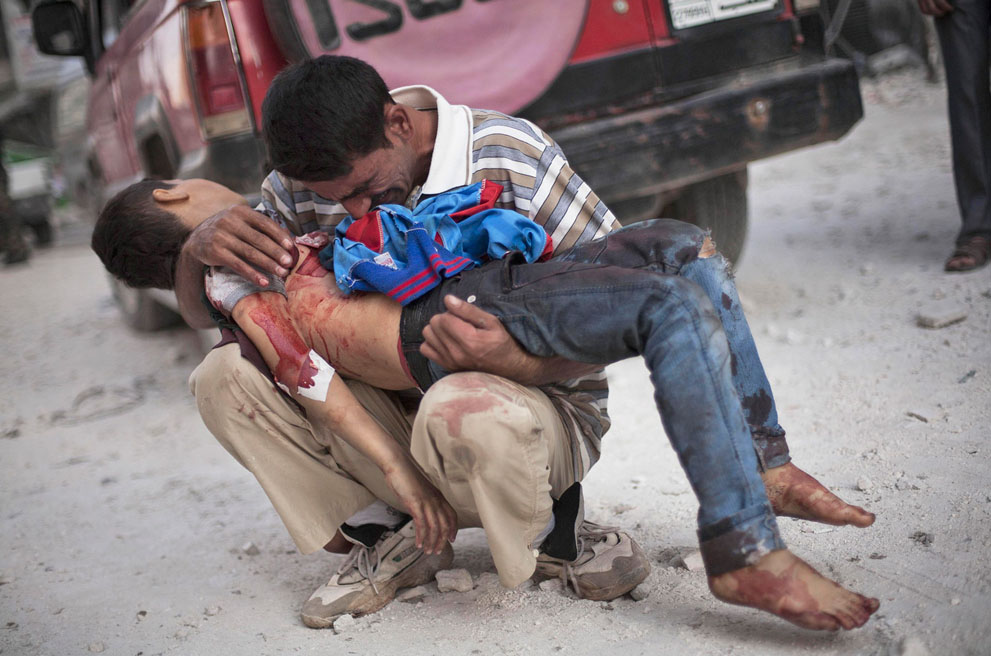
\includegraphics[width=\textwidth, height=7cm]{syria.jpg}
    %\end{center}
%}




  


\end{document}

    \frame{\frametitle{}
    }
    \frame[t]{\frametitle{Exercise }
    }

    \frame[t]{
      \begin{block}{Exercise}
      \end{block}
      \noindent
      \textbf{Solution.}\nopagebreak\vspace{2in}
    }

      \bigskip
      \medskip
      \smallskip

      \begin{center}
       \includegraphics[width=\textwidth]{.png}
      \end{center}

      \pause
      \begin{block}{}
      \end{block}

      \begin{columns}
        \begin{column}{0.5\textwidth}
        \end{column}
        \begin{column}{0.5\textwidth}
        \end{column}
      \end{columns}
  }

